\lecture{Condensed Summaries}{Conv Nets: A Modular Perspective}{December 21}


\p \href{https://colah.github.io/posts/2014-07-Conv-Nets-Modular/}{From this post on Colah's Blog}. 

\myspace The title is inspired by the following figure. Colah mentions how groups of neurons, like $A$, that appear in multiple places are sometimes called \textbf{modules}, and networks that use them are sometimes called modular neural networks. You can feed the output of one convolutional layer into another. With each layer, the network can detect higher-level, more abstract features.
\myfig[0.3\textwidth]{ColahConv2.PNG}
\begin{compactitem}[$\longrightarrow$]
	\item Function of the $A$ neurons: compute certain \textit{features}.
	
	 \item Max pooling layers: kind of ``zoom out''. They allow later convolutional layers to work on larger sections of the data. They also make us invariant to some very small transformations of the data.
\end{compactitem}



\lecture{Condensed Summaries}{Understanding Convolutions}{December 21}


\p \href{https://colah.github.io/posts/2014-07-Understanding-Convolutions/}{From Colah's Blog}. 

\p \blue{Ball-Dropping Example}. The posed problem:
\begin{footnotesize}
\begin{quote}
	Imagine we drop a ball from some height onto the ground, where it only has one dimension of motion. How likely is it that a ball will go a distance c if you drop it and then drop it again from above the point at which it landed?
\end{quote}
\end{footnotesize}

\begin{figure}[h!]
	\centering
	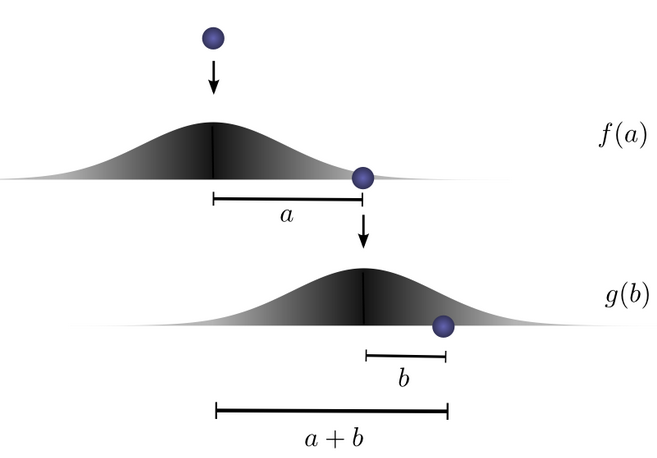
\includegraphics[width=0.35\textwidth]{ColahBall.PNG}
	\hspace{2cm}
	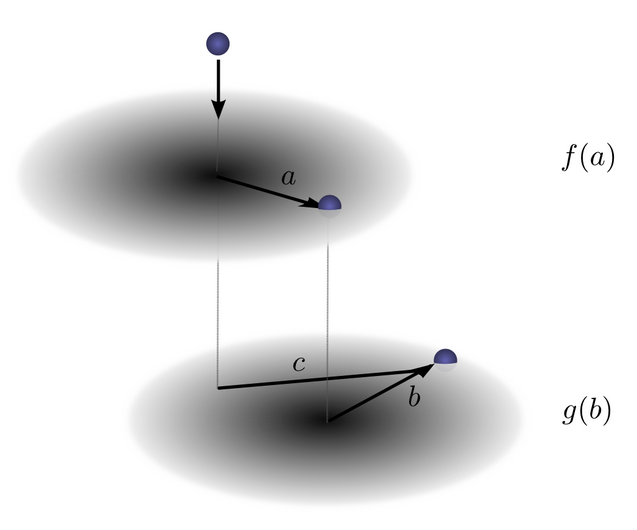
\includegraphics[height=0.25\textwidth]{ColahBall3.PNG}
\end{figure}

From basic probability, we know the result is a sum over possible outcomes, constrained by $a + b = c$. It turns out this is actually the definition of the convolution of $f$ and $g$. 
\begin{align}
	\mathrm{Pr(a + b = c)} &= \sum_{a + b = c} f(a) \cdot g(b) \\
	(f * g)(c) &= \sum_{a + b = c} f(a) \cdot g(b)\\
	&= \sum_a f(a) \cdot g(c - a)
\end{align}

\myspace
\p \blue{Visualizing Convolutions}. Keeping the same example in the back of our heads, consider a few interesting facts. 
\begin{itemize}
	\item \textbf{Flipping directions}. If $f(x)$ yields the probability of landing a distance $x$ away from where it was dropped, what about the probability that it was dropped a distance $x$ from where it \textit{landed}? Apparently\footnote{Not entirely sold on the generalization of this, or even how true it is here.} it is $f(-x)$. 
	
	\myfig[0.3\textwidth]{ColahBall2.PNG}
	
	\item Above is a visualization of one term in the summation of $(f * g)(c)$. It is meant to show how we can move the bottom around to think about evaluating the convolution for different $c$ values. 
\end{itemize}
We can relate these ideas to image recognition. Below are two common kernels used to convolve images with. 
\begin{figure}[h!]
	\centering
	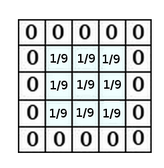
\includegraphics[width=0.15\textwidth]{ColahKernel1.PNG}
	\hspace{2.5cm}
	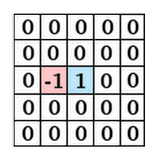
\includegraphics[height=0.15\textwidth]{ColahKernel2.PNG}
\end{figure}

On the left is a kernel for \textit{blurring} images, accomplished by taking simple averages. On the right is a kernel for \textit{edge detection}, accomplished by taking the difference between two pixels, which will be largest at edges, and essentially zero for similar pixels.






























\end{document}
